\section{Główna pętla programu} %OK
\begin{figure}[H]
	\centering
	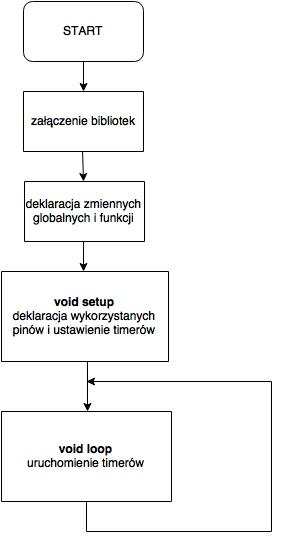
\includegraphics[scale=0.65]{mainProgram.jpg}
	\caption{Główna pętla programu}
\end{figure}
Struktura programu napisanego w języku Arduino przypomina strukturę charakterystyczną dla języka C/C++. Na początku pliku zadeklarowane zostają wykorzystane biblioteki. W tym przypadku użyto trzech:
\begin{itemize}
\item \textit{Simple Time}- tworzenie niestandardowych timerów,
\item \textit{Liquid Crystal}- obsługa wyświetlacza LCD,
\item \textit{OneWire}- odczyt danych z urządzeń korzystających z technologii OneWire.
\end{itemize}
Następnie utworzone zostają zmienne globalne, dostępne dla wszystkich funkcji. 
Przechowują one wartości nastaw regulatorów, aktualne odczyty oraz numery wykorzystanych wejść/wyjść mikrokontrolera. Następnie zostają zdefiniowane funkcje utworzone w programie.

Program składa się na dwie główne części opisane i zaprezentowane na Rysunku nr. \ref{ArduinoPodstawoweFunkcje}. W wykonywanej tylko raz funkcji \textit{void setup(void)} piny Arduino zostały ustawione jako wyjścia lub wejścia. Wejściem został jedynie pin nr. 8 podłączony do termometru. Wywołana została funkcja \textit{setLCD\_start()}, odpowiadająca za wyświetlenie na ekranie informacji, których odświeżanie nie będzie konieczna. Ostatnią rzeczą wykonaną na tym etapie jest utworzenie nowych timerów odpowiadających za:
\begin{itemize}
\item regulację temperatury co 1 sekundę,
\item wysyłanie danych co 1 sekundę,
\item odbieranie danych co 2 sekundy.
\end{itemize}

W nieustannie wykonywanej funkcji \textit{void loop(void)} zadano silnikom pracę z maksymalną prędkością obrotową. Została wykonana metoda \textit{timer.run} uruchamiająca pracę wcześniej utworzonych timerów.

W kolejnych sekcjach opisano działanie funkcji wywoływanych przez timery oraz obsługę urządzeń peryferyjnych.

\section{Odbiór danych}%OK
Do komunikacji między urządzeniami wykorzystano moduł Bluetooth, połączony z Arduino przez port szeregowy UART. Do obierania danych przesłanych przez urządzenie mobilne utworzono funkcję \textit{bluetoothReceive()}, wywoływaną przez timer co 2 sekundy. Wejście RX Arduino zostało połączone z wyjściem TX modułu. Pozostałe piny połączono adekwatnie. Komunikacja odbywa się poprzez przesłanie ramki danych o wyznaczonym symbolu rozpoczęcia i zakończenia ciągu danych. Struktura ramki została przedstawiona na rysunku \ref{ramka1}.
\begin{figure}[H]
\centering
\Huge "tXpXjXdXrXhXmX/n"
\label{ramka1}
\caption{Ramka komunikacji od urządzenia mobilnego do Arduino}
\end{figure}
Znaki \textit{X} oznaczają wartości parametrów. Przez małe litery oznaczono informację o początku danego parametru:
\begin{itemize}
\item \textit{t}- temperatura zadana,
\item \textit{p}- wzmocnienie części proporcjonalnej,
\item \textit{i}- wzmocnienie części inercyjnej,
\item \textit{d}- wzmocnienie części różniczkującej,
\item \textit{r}- typ regulatora, PID lub histerezowy,
\item \textit{h}- wartość histerezy,
\item \textit{m}- moc regulatora histerezowego,
\item \textit{/n}- zakończenie ramki.
\end{itemize}
Na początku działania funkcji odbioru danych zostają utworzone zmienne dla każdego określonego znaku charakterystycznego i parametru. W celu ułatwienia konwersji danych, dla parametrów utworzono zmienne typu string oraz int lub float.

Przed rozpoczęciem pobierania wykonane zostaje polecenie sprawdzające czy bufor portu szeregowego przechowuje jakieś dane. Jeśli tak, to zostaje wykonane polecenie \\ \textit{Serial.readStringUntil('/n')}, zapisujące wszystkie znaki przechowywane przez bufor, aż do napotkania znaku zakończenia ramki ,,/n''. Jeśli długość otrzymanego ciągu znaków jest równa lub większa od minimalnej długości ramki, to rozpoczyna się proces obróbki danych.

Kolejnym krokiem jest wykonanie się pętli \textit{for}, której zadaniem jest znalezienie wszystkich określonych znaków charakterystycznych i przypisanie ich położenia w ciągu znaków do zmiennej o tym samym symbolu co znak, którego położenie określa.

Następnie za pomocą polecenia \textit{String.substring(a,b)} z otrzymanego ciągu znaków zostają wycięte części odpowiadające wartościom parametrów, które zostają zapisane do zmiennych string. Aby zamienić ciągi znaków na liczby, użyto metod \textit{String.toInt()} oraz \textit{String.toFloat}. Powstałe wartości liczbowe przypisano do zmiennych globalnych.
\newpage
\section{Regulacja temperatury}%jest ok
\begin{figure}[H]
	\centering
	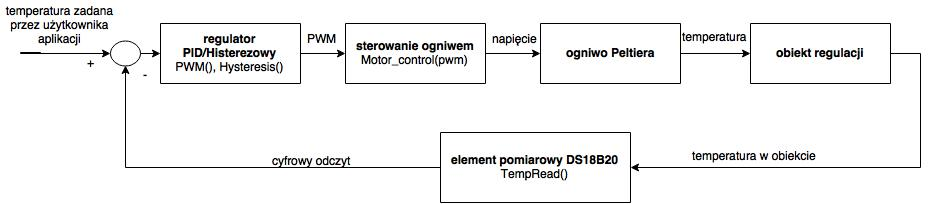
\includegraphics[scale=0.45]{regulacjatemp.jpg}
	\caption{Schemat regulacji temperatury}
\end{figure}
Funkcja \textit{void regulation()} wywoływana przez drugi timer jest odpowiedzialna za proces regulacji temperatury, na który składa się: odczyt aktualnej wartości temperatury, obliczenie sygnału sterującego PWM oraz sterowanie ogniwem za pomocą funkcji przedstawionych na poniższym listingu.
\lstset{language=C++}
\lstset{
	basicstyle=\footnotesize,
	breaklines=true,
	showspaces=false,
	%inputencoding=utf8, 
	%extendedchars=\true,
	literate={ą}{{\k{a}}}1
             {Ą}{{\k{A}}}1
             {ę}{{\k{e}}}1
             {Ę}{{\k{E}}}1
             {ó}{{\'o}}1
             {Ó}{{\'O}}1
             {ś}{{\'s}}1
             {Ś}{{\'S}}1
             {ł}{{\l{}}}1
             {Ł}{{\L{}}}1
             {ż}{{\.z}}1
             {Ż}{{\.Z}}1
             {ź}{{\'z}}1
             {Ź}{{\'Z}}1
             {ć}{{\'c}}1
             {Ć}{{\'C}}1
             {ń}{{\'n}}1
             {Ń}{{\'N}}1
	}
\begin{lstlisting}
void regulation() {
  temperatureReading = TempRead();	//odczyt temperatury
  if (regulatorType == 0) {	
    pwm = PID(temperatureSetpoint, temperatureReading, millis(), kp , ki, kd); //wywołanie własnego regulatora PID
  }
  else {	//wywołanie regulatora histerezowego
    pwm = HIST(temperatureSetpoint, temperatureReading, hysteresis, power);
  }
  Motor_Control(pwm);	//funkcja sterująca ogniwem
}
\end{lstlisting}
Proces rozpoczyna się od wywołania funkcji odczytującej temperaturę. Następnie zostaje sprawdzony typ regulatora zapisany w postaci cyfry. W zależności od wyboru użytkownika, zostaje użyty regulator histerezowy lub PID. Wartości parametrów każdego z nich mogą zostać dostosowane w aplikacji mobilnej. Otrzymany sygnał sterujący zostaje przekazany funkcji sterującej ogniwem.
\subsection{Odczyt temperatury}
Do odczytu temperatury zmierzonej przez termometr cyfrowy DS18B20 użyto biblioteki \textit{OneWire} oraz funkcji dedykowanej dla wybranego termometru, dostępnej na stronie producenta Arduino. Na początku programu utworzono obiekt \textit{OneWire ds(8)}, któremu zostało przypisane ósme wejście mikrokontrolera.

Funkcja rozpoczyna swoje działanie od wyszukania urządzeń podłączonych do linii OneWire. Znaleziony adres zostaje przechowany w zmiennej. Następnie za pomocą polecenia \textit{ds.select(addr)}, zostaje nawiązana komunikacja z wybranym urządzeniem. W kolejnym etapie do termometru zostaje wysłane wymuszenie odczytu danych. Termometr zapisuje do \textit{brudnopisu} wartość uzyskaną od wbudowanego przetwornika analogowo-cyfrowego. Dane przechowywane w \textit{brudnopisie} mogą zostać odczytane w każdej chwili. Jeśli nie zostało wcześniej wykonane polecenie konwersji, to termometr zwróci ostatnią odczytaną wartość. Czas trwania konwersji danych zależy od rozdzielczości, jaką chce osiągnąć użytkownik. Do termometru zostaje przesłana wartość \textit{0xBE}, w odpowiedzi na którą urządzenie udostępnia pomiar. W celu uzyskania największej rozdzielczości, należy odczytać 12 bitów danych, które następnie zostają zamienione na pomiar temperatury.

\subsection{Regulator PID} %to ok
Regulator PID zbudowany jest z 3 członów: proporcjonalnego (P), inercyjnego (I) i różniczkującego (D). Zaimplementowany regulator posiada funkcję anti-windup. Najważniejszymi argumentami funkcji są: aktualna temperatura, wartość zadana oraz parametry. Język Arduino nie posiada zaimplementowanego działania całkowania ani różniczkowania, dlatego działania te musiały zostać uproszczone. Użyto całkowania i różniczkowania numerycznego. Regulacja wykonywana jest przez układ dyskretny.

\begin{lstlisting} 
int PID(int setpointTemperature, float currentTemperature, float actualTime, int kp, int ki, int kd) {
  float maximum = 255;
  float minimum = -255;
  float static integral = 0;
  float static previousTime = 0;
  float static previousError = 0;
  float static previousOutput=0;
  float error = setpointTemperature - currentTemperature;
  float dt = (float)(actualTime - previousTime);
  dt=dt/60000; //przeskalowanie czasu na minuty
  if(previousOutput>-255&&previousOutput<255){	//anty-windup
    integral = integral + (error * dt);	//człon całkujący
  }
  if (integral > 1) {	//ograniczenie całki
    integral = 1;
  }
  else if (integral < -1) {
    integral = -1;
  }
  float derivative = (error - previousError) / dt;	//człon różniczkujący
  previousError = error;
  previousTime = actualTime;
  int output = kp * error + ki*integral + kd * derivative; //sygnał wyjściowy
  previousOutput=output;
  if (output >= maximum){	//ograniczenie wartości wyjścia
    output = maximum;
  }
  else if ( output <= minimum){
    output = minimum;
  }
  return output;
}
\end{lstlisting}
Na potrzeby prawidłowego działania regulatora, utworzono zmienne określające maksymalne wartości wyjścia regulatora oraz zmienne statyczne, przechowujące dane potrzebne w kolejnych wywołaniach funkcji. Na początku zostaje obliczony błąd regulacji- \textit{error} oraz czas- \textit{dt} jaki upłynął od poprzedniego wywołania funkcji. Uzyskana wartość czasu zostaje przeskalowana do minut. Następnie sprawdzone zostaje jaką wartość przyjęła poprzednia instancja regulatora. Jeśli mieści się ona w zakresie od -255 do 255, to zostaje obliczona nowa wartość części inercyjnej regulatora. Takie rozwiązanie zostało potraktowane jako zaimplementowanie systemu anty-windup. Dzięki tej funkcji, człon całkujący nie będzie dalej narastał, gdy wyjście ma wartość maksymalną. Dodatkowo nałożono ograniczenie wartości maksymalnej członu całkującego. Wartość całki została uproszczona do sumy poprzedniej wartości całki i błędu pomnożonego przez czas \textit{dt}. W kolejnym kroku, sprawdzane jest, czy wartość całki mieści się w określonym zakresie. W przypadku niespełnienia warunku, całka zostaje ograniczona.Człon różniczkujący został obliczony przez różnicę aktualnego błędu regulacji i poprzedniego błędu podzielonego przez \textit{dt}. Sposób zapisu uproszczonych działań wzorowany jest na źródle [1] oraz przykładzie, który przedstawiono podczas zajęć dydaktycznych. Wartość błędu i aktualny czas zostają zapisane do zmiennych statycznych.

Wyjście regulatora zostaje wyznaczone przez pomnożenie obliczonych członów przez odpowiadające im wzmocnienia, które następnie zostają zsumowane. Wyjście regulatora zostaje ograniczone do przedziału od -255 do 255, w celu nieprzekroczenia maksymalnej wartości sygnału PWM.

\subsection{Regulator histerezowy}%jest ok
Regulacja histerezowa polega na regulowaniu temperatury poprzez ustalenie zakresów, dla których obiekt grzewczy będzie włączony lub wyłączony. Wartości mogą zostać wybrane przez użytkownika za pomocą aplikacji mobilnej. Gdy temperatura spadnie poniżej zadanej histerezy, obiekt grzewczy zostaje załączony i ogrzewa pomieszczenie, aż osiągnie wartość mieszczącą się w zakresie histerezy. Następnie jest wyłączony, aż do ponownego wyjścia temperatury z zakresu.
\begin{lstlisting}
int HIST(int setpointTemperature, float currentTemperature, float hystValue, int powerValue)
\end{lstlisting}
%\subsection{Regulator trójstawny}%jest ok
%Regulator trójpołożeniowy jest bardzo podobny do histerezowego. Jedyną różnicą jest to że oprócz pełnienia funkcji grzewczej, może on również chłodzić. W tym przypadku regulator ma określone aż trzy stany, gdzie podczas pierwszego ogrzewa, w drugim zostaje wyłączony, a w trzecim pracuje w przeciwnym kierunku niż pierwszy.
\subsection{Sterowanie ogniwem}%jest ok
Na wejście funkcji sterowania ogniwem wysłany zostaje sygnał PWM, obliczony przez aktualnie wybrany przez użytkownika regulator.
\begin{lstlisting}
void Motor_Control(int Speed)
{
  if (Speed > 0){	//włączenie ogrzewania
    digitalWrite(IN2, LOW);
    digitalWrite(IN1,  HIGH);
    analogWrite(ENA, Speed);
  }
  else if (Speed < 0){	//włączenie chłodzenia
    Speed = Speed * (-1);
    digitalWrite(IN2, HIGH);
    digitalWrite(IN1, LOW);
    analogWrite(ENA, Speed);
  }
  else {	//ogniwo wyłączone
    digitalWrite(IN1, LOW);
    digitalWrite(IN2, LOW);
  }
}
\end{lstlisting}
Wybór funkcji grzewczej lub chłodniczej odbywa się poprzez zadanie odpowiednich stanów logicznych na wejścia \textit{IN1} i \textit{IN2} sterownika. Możliwe kombinacje to:
\begin{itemize}
\item chłodzenie- \textit{IN1} stan wysoki, \textit{IN2} stan niski,
\item ogrzewanie- \textit{IN1} stan niski, \textit{IN2} stan wysoki,
\item zatrzymanie pracy ogniwa- \textit{IN1} i \textit{IN2} w stanie niskim.
\end{itemize}
Sterowanie mocą ogniwa odbywa się poprzez wysłanie sygnału PWM o częstotliwości w zakresie od 0 do 255 na wejście \textit{ENA} sterownika.

Na początku funkcji sprawdzana jest wartość sygnału PWM. Jeśli sygnał ma wartość większą od zera, to zostają wysłane sygnały z drugiej kombinacji. W przypadku, gdy sygnał przyjmuje wartości ujemne, musi zostać wyznaczona jego wartość bezwzględna i dopiero ta może zostać wysłana. Piny sterujące zostają ustawione w pierwszej kombinacji. W przypadku nie spełnienia żadnego z warunków, na oba wejścia sterujące wysyłany jest stan niski, zatrzymujący pracę ogniwa.

\section{Wysyłanie danych} %jest ok
Funkcja wysyłania danych \textit{bluetoothSend()} wykonywana jest w odstępach czasu wynoszących 1 sekundę. Odpowiedzialna jest za wyświetlenie aktualnych pomiarów na wyświetlaczu oraz przekazaniu ich urządzeniom mobilnym. Komunikacja odbywa się przez port szeregowy UART, połączony z modułem Bluetooth. Dane tekstowe zostają zawarte w ramce komunikacyjnej i wysłane pomocą polecenia \textit{Serial.print("tekst")}.

Ramka przekazywana w tym kierunku różni się od opisywanej poprzednio długością, ze względu na większą ilość przekazywanych parametrów, które zostały opisane poniżej.
\begin{figure}[H]
\label{ramkaOdArduino}
\centering
\Huge "tXsXpXlXiXdXrXhXmX/n"
\caption{Ramka przesyłana z mikrokontrolera do urządzenia mobilnego}
\end{figure}
Przez duże znaki oznaczono wysyłane wartości parametrów. Małe litery przekazują informację o rozpoczęciu danego segmentu ramki. Na przekazywane parametry składają się:
\begin{itemize}
\item \textit{t}- temperatura odczytana przez termometr,
\item \textit{s}- temperatura zadana
\item \textit{p}- sygnał PWM,
\item \textit{k}- wzmocnienie części proporcjonalnej,
\item \textit{i}- wzmocnienie części inercyjnej,
\item \textit{d}- wzmocnienie części różniczkującej,
\item \textit{r}- typ regulatora,
\item \textit{h}- wartość histerezy,
\item \textit{m}- moc regulatora histerezowego,
\item \textit{/n}- zakończenie ramki.
\end{itemize}
Interfejs użytkownika opisany w kolejnym rozdziale, pozwala na wyświetlanie wszystkich aktualnych nastaw, dlatego niektóre wartości przekazywane są w obu kierunkach.

Ostatnią wykonaną w tym timerze funkcją jest zaktualizowanie danych wyświetlanych na ekranie LCD.
\subsection{Aktualizacja wyświetlacza LCD} %jest ok
Obiekt, którego metody używane są do sterowanie wyświetlaczem, został zadeklarowany na samym początku programu. Linię kodu zamieszczono poniżej.
\begin{lstlisting}
LiquidCrystal lcd(2,3,4,5,6,7);
\end{lstlisting}
Kolejne cyfry odpowiadają wyjściom Arduino przypisanym do pinów \textit{RS, E, D4, D5, D6, D7} ekranu.
Proces wstępnej konfiguracji ekranu został przedstawiony w poniższym listingu.
\begin{lstlisting}
void setLCD_start() {
  lcd.begin(16, 2);
  lcd.setCursor(0, 0);	//ustawienie pozycji kursora
  lcd.print("Reading "); //wyświetlenie tekstu
  lcd.setCursor(15, 0);
  lcd.print("C");
  lcd.setCursor(0, 1);
  lcd.print("Setpoint  ");
  lcd.setCursor(15, 1);
  lcd.print("C ");
}
\end{lstlisting}
Obiekt lcd został zadeklarowany jako wyświetlacz o 2 wierszach i 16 kolumnach, czyli w sumie 32 znakach. Położenie kursora zostało ustawione w odpowiednie punkty ekranu, a następnie wyświetlono pożądany tekst. W pierwszym rzędzie ekranu wyświetlono \textit{Reading}, a w drugim \textit{Setpoint}. Na końcu obu linii umieszczono znak stopni Celsjusza. Wcześniejsze przygotowanie ekranu za pomocą tej funkcji pozwala na ograniczenie ilości danych, cyklicznie wysyłanych do wyświetlacza.

W kolejnych wywołaniach trzeciego timera wykonywana jest funkcja \textit{setLCD(temperatureSetpoint, temperatureReading)} aktualizująca wyświetlaną wartość zadaną i pomiar temperatury.
\begin{lstlisting}
  lcd.setCursor(9, 0);
  lcd.print(temp,1);
  lcd.setCursor(9, 1);
  lcd.print((float)setpoint,1);
\end{lstlisting}